\appendix
\chapter{Appendix: Meeting protocols} \label{sec:appendix}

\section{Meeting 01 - 15.10.2012}
The first meeting started with a presentation of the work of the \emph{Frauenhofer Institute}, which is part of the \emph{Frauenhofer Society}. The Frauenhofer Society is a German research organization with $60$ institutes spread throughout Germany, each focusing on different fields of applied science (as opposed to the Max Planck Society, which works primarily on basic science).

The course is guided by Prof. Dr. Ina Schieferdecker. Our project group works with three computer scientists from the Frauenhofer Fokus institute in Berlin (Tom Ritter, Christian Hein and Michael Wagner).

At this meeting, we first got a general introduction to model driven engineering. Therefore we reviewed learning methods of abstraction to focus on creating and exploiting domain models (that is, abstract representations of the knowledge and activities that govern a particular application domain), rather than on the computing (or algorithmic) concepts. We also got a small overview over the main software development processes (waterfall model, v-model and so on). Our first task for the following week should be to create an UML diagram with Papyrus for a generic firm.

\section{Meeting 02 - 22.10.20120}
We presented all solutions for the task with the firm. There where surprisingly different solutions for the task. So there were actually no right or wrong solutions. For example: An employee was a full-time, half-time or even external worker. We modeled that with having an enumeration containing those items. Others used inheritance to model such a system. The next task was to create an UML profile for this firm.

\section{Meeting 03 - 29.10.2012}
The solutions of the UML profile were not as expected. All teams had different profiles and although there is no right and wrong again everybody had problems with Papyrus. In many cases Eclipse just did not react to changes in the diagram or did not do the expected operations. Only one person had no problems with Eclipse, so this person presented its profile. So the difficulty was not to create the profile, but to get this plugin working.

\section{Meeting 04 - 05.11.2012}
The first meetings were like an introduction to model based engineering. We got a few tasks to do. In this meeting the project tasks were presented. There were a bunch of tasks. In most cases a tool for a special case was needed and so we should implement it. We wanted to take the Sonar task and we were lucky, because nobody else wanted to take this task. With the teams we made a small brainstorming to get a feeling for the task. In this brainstorming we collected our knowledge about static code analysis and especially Sonar. Because of the fact some team members already had worked with Sonar, they gave us a short introduction to code analysis with Sonar.

The task for the following week was to install and test Sonar and the Modelbus repository, which is a system containing models and source code, that should be analyzed with Sonar (that was our task). Another task was to work out some first requirements.

\section{Meeting 05 - 12.11.2012}
We presented the requirement list, which of course was not specific enough. We simply did not have much knowledge about the task and about plugin development for Sonar. Other teams had the same issue, their results were not specific as well.

The task for the following meeting was to specify the requirements more and to provide a first architecture concept. You can find the new requirement list here.

\section{Meeting 06 (Hackathon) - 23.11.2012}
The weekly meeting at university was not taking place this week, so we decided to meet and work together in the team. We therefore organized a hackathon, where we installed the software (some had build problems during the installation of the components). We also worked out an architecture concept and created a few diagrams to show our progress.

\section{Meeting 07 - 26.11.2012}
We presented our new requirements and the architecture. Our architecture concept (\autoref{fig:architecture}) and the workflow (\autoref{fig:sequence}) was regarded to be good enough, so we are good to start the development of the plugin. From now on, we focus on more technical tasks.

\begin{figure}[!htbp]
\centering
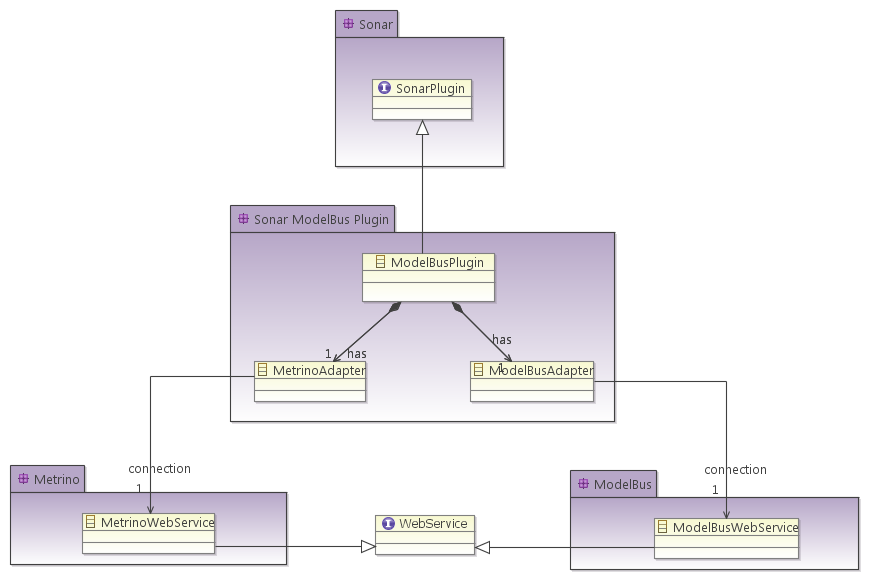
\includegraphics[width=\textwidth]{architecture}
\caption{Architecture of the Sonar plugin}
\label{fig:architecture}
\end{figure}

\begin{figure}[!htbp]
\centering
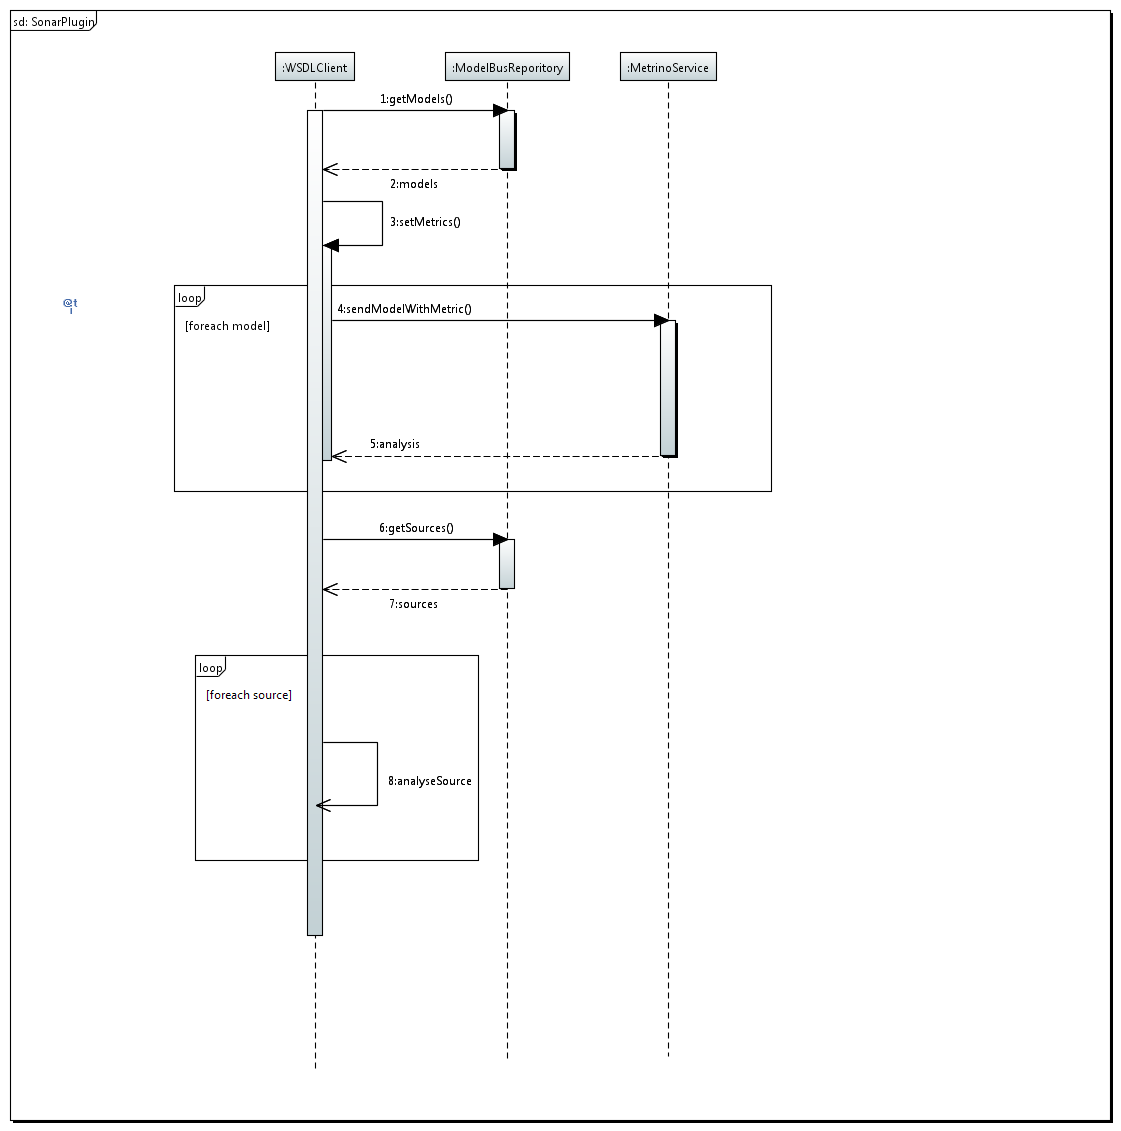
\includegraphics[width=\textwidth]{sequencediagramm}
\caption{Sequence diagram, showing the activity of our plugin}
\label{fig:sequence}
\end{figure}

\section{Meeting 08 - 03.12.2012}
At this meeting, we presented the current results. The result is, that our WSDL client can connect to the Modelbus repository. The Modelbus service is now successfully driven on our test system and it is planned to connect successfully to the Metrino service.

In the discussion with the project head members, they suggested to use a customer instead of a WSDL client to connect to the Modelbus repository. The customer is a type of client service, which do not communicate with the service with WSDL but instead connects directly to the Java interface of Modelbus.

After discussing this point, other questions raised concerning object-oriented metrics for models:

\begin{itemize}
\item What kind of properties can be analysed on object-oriented code?
\item Into what extend can analyse of object-oriented code applied to object-oriented models?
\item Requirement: Sonar shall be capable to analyse object-oriented code, too. These analysis shall be applied to models, too.
\end{itemize}

\section{Meeting 09 - 10.12.2012}
At the beginning of this meeting, we presented our current results and reported some problems. Our biggest problem was, that during the installation process of Metrino, a lot of Eclipse libraries must be installed by hand. As we reported this problem to the organizer of this course, he answered that in theory, a manually installation of Eclipse libraries is not required but in practice, some Eclipse libraries must be integrated.

Another discussion point was, that we wrote a message to the developers of Modelbus and Metrino and asked them about a consumer, which can connect to the Modelbus repository without an own WSDL client. We tried it with the consumer but unfortunately, it did not work. Therefore, we connected manually to the Modelbus repository. Additionally, we wanted to connect to the Metrino service but we discovered, that Metrino can just be reached locally. Even in the same network, the connection did not work.

We explained our organizer, that we still not know how to send our metrics to Metrino, thus we need an API documentation.

We told our organizer about the complex installation process of Modelbus: To configure Modelbus, the Modelbus-Root for the local service must be pointed to a config file, which points to a remote server.

An additional discussion point was, that there is no list of dependent libraries for the configuration of Modelbus.

Our organizer told us, that he will send us a front-end for the Metrino service, so that we can understand which metrics Metrino can use.

The last point of discussion was, that one of our team members had the idea, that models can be translated into Java code, which can then be analyzed statically by Sonar. But this would break a requirement, which says that a model must be analyzable, too.

\section{Meeting 10 - 17.12.2012}
During the last week, we discovered the problem that the checkout of the models from the Modelbus repository did not work. We always got an exception \texttt{ServiceConstructionException}. In the standalone version of our plugin, the checkout worked. We explained this error to our supervisor and he explained that we must send this problem to their mailing list. Then, we asked them a few questions about some functions of the Metrino service, which occurred during the work with it.

\section{Meeting 11 - 07.01.2013}
We reported the current state of our plugin project. Now, the Metrino service runs on our own server on \emph{openstoryboard.org}. The problem is, that we want to reach the service from the outside of the network. Therefore we need a proxy.

We checked in some models into the Modelbus repository. We explained that we still get some exceptions during the checkout of some models from the repository. Because of that, we asked for the source code of Modelbus so that we can debug the code. The supervisor suggested, that one member of our team could visit him the next day at Frauenhofer so that they can debug our code together.

Additionally, we explained that Sonar is not designed to analyze code in different languages within one process. To be able to analyze different kind of languages, a separate module must be run for each language and therefore, cannot be done within one plugin. To analyze different languages, we must write a plugin for each language which is not the object of our plugin project.

\section{Meeting 12 - 14.01.2013}
To summarize our work, we explained how our plugin works and for what it is designed for. We explained, that we checkout models from the Modelbus repository, that we send them with metric descriptions to the Metrino service and get the result file and finally, that we already have a module, which can visualize results in Sonar.

The next task is to build a SMM Parser which can read the result SMM file, which we get from the Metrino service, and to store the results in data structures, which are read by Sonar.

The example SMM files, which we got from our supervisor, computed two metrics: the number of classes and the number of packaged of a metric. We have seen that there are more than just one result value for a metric computation. Therefore, we must know which one of them is the newest one. Our supervisor explained, that the XSD of the SMM file explains that each result can have a time stamp so that we can see easily, which one is the newest metric result.

\section{Meeting 13 - 21.01.2013}
This week, the meeting did not take place. Our group organized a Skype meeting where we discussed the results of our tasks and what are the tasks for the following week. The visualization of results in Sonar still not works properly and we must go on with these tasks. Additionally, we updated our requirements list. We discussed about the SMM parser, which was built until this day and realized, that there are some errors which must be fixed this week, because next week, we want to put all modules of the Sonar plugin together.

\section{Meeting 14 (Hackathon) - 26.01.2013}
Today, we have a hackathon. We have a lot of results for each little module of our plugin project and we want to put them all together.

At first, we integrated our SMM parser into our plugin. We changed the parser a little bit. We added an input stream to the Resource object, because by doing this we can send the checked out models directly from the main application to our parser instead of saving the checked out models in a file.

Afterwards, we work on metrics for Metrino. We have got two example metrics, but we want to define some more metrics. We have written them in OCL. For a few weeks, our supervisor sent us a Modelbus eclipse project where they can create metrics within a GUI perspective. In some cases, we got an exception so that we started to write metrics in OCL by hand.

Finally, we discussed about the next tasks and steps.

\section{Meeting 15 - 28.01.2013}
We reported the current state of our project. There are still two requirements, which are not satisfied. One metric is, that we analyze more than just one language within our plugin, but in discussion with the developers of Sonar, we got to know, that this is not possible within a single Sonar plugin. The second requirement is the question, how many other metrics we shall create to analyze models.

We thought about two ways: One way is to write a lot of metrics by hand and statically integrate them in our plugin. Thus, if a user wants to have additional metrics, he or she must insert them manually. Another way is to write an extension for our plugin so that the user can write some metrics and our plugin can load them dynamically. In general, Sonar plugin uses metrics which are added manually. This means that if we want our plugin to be statically load the metrics, we must write them all by hand into our classes, thus we must know all metrics a user possibly want to analyze in Sonar or the user have in the SMM files. We decided to write a mechanism to load dynamically metrics.

Our supervisor recommended us to take all metrics, which Sonar uses to analyze source code in Java. Therefore, we must examine which of the metrics in Sonar we can adapt to analyze models.

\section{Meeting 16 - 4.02.2013}
The last week, we tried to find out how we can dynamically load metrics into our plugin, so that a user do not have to write them by hand. We explained how much we could find out and additionally, we presented the first version of our documentation and got some constructive criticism. 

\section{Meeting 17 - 11.02.2013}
In the last meeting, we presented the current state and which sub-tasks are left to finish the plugin development. We explained that we still have problems to visualize the results of Metrino in Sonar and which exceptions we got. Our supervisor told us to meet him after the lecture so that we can take a look at the problem. Finally, we presented him the current version of our documentation. There are some good points, for example that the software architecture should be the main part in our documentation (but we placed it after the installation manual).